\documentclass[twoside]{book}

% Packages required by doxygen
\usepackage{fixltx2e}
\usepackage{calc}
\usepackage{doxygen}
\usepackage[export]{adjustbox} % also loads graphicx
\usepackage{graphicx}
\usepackage[utf8]{inputenc}
\usepackage{makeidx}
\usepackage{multicol}
\usepackage{multirow}
\PassOptionsToPackage{warn}{textcomp}
\usepackage{textcomp}
\usepackage[nointegrals]{wasysym}
\usepackage[table]{xcolor}

% Font selection
\usepackage[T1]{fontenc}
\usepackage[scaled=.90]{helvet}
\usepackage{courier}
\usepackage{amssymb}
\usepackage{sectsty}
\renewcommand{\familydefault}{\sfdefault}
\allsectionsfont{%
  \fontseries{bc}\selectfont%
  \color{darkgray}%
}
\renewcommand{\DoxyLabelFont}{%
  \fontseries{bc}\selectfont%
  \color{darkgray}%
}
\newcommand{\+}{\discretionary{\mbox{\scriptsize$\hookleftarrow$}}{}{}}

% Page & text layout
\usepackage{geometry}
\geometry{%
  a4paper,%
  top=2.5cm,%
  bottom=2.5cm,%
  left=2.5cm,%
  right=2.5cm%
}
\tolerance=750
\hfuzz=15pt
\hbadness=750
\setlength{\emergencystretch}{15pt}
\setlength{\parindent}{0cm}
\setlength{\parskip}{0.2cm}
\makeatletter
\renewcommand{\paragraph}{%
  \@startsection{paragraph}{4}{0ex}{-1.0ex}{1.0ex}{%
    \normalfont\normalsize\bfseries\SS@parafont%
  }%
}
\renewcommand{\subparagraph}{%
  \@startsection{subparagraph}{5}{0ex}{-1.0ex}{1.0ex}{%
    \normalfont\normalsize\bfseries\SS@subparafont%
  }%
}
\makeatother

% Headers & footers
\usepackage{fancyhdr}
\pagestyle{fancyplain}
\fancyhead[LE]{\fancyplain{}{\bfseries\thepage}}
\fancyhead[CE]{\fancyplain{}{}}
\fancyhead[RE]{\fancyplain{}{\bfseries\leftmark}}
\fancyhead[LO]{\fancyplain{}{\bfseries\rightmark}}
\fancyhead[CO]{\fancyplain{}{}}
\fancyhead[RO]{\fancyplain{}{\bfseries\thepage}}
\fancyfoot[LE]{\fancyplain{}{}}
\fancyfoot[CE]{\fancyplain{}{}}
\fancyfoot[RE]{\fancyplain{}{\bfseries\scriptsize Generated on Tue Feb 10 2015 11\+:10\+:27 for My Project by Doxygen }}
\fancyfoot[LO]{\fancyplain{}{\bfseries\scriptsize Generated on Tue Feb 10 2015 11\+:10\+:27 for My Project by Doxygen }}
\fancyfoot[CO]{\fancyplain{}{}}
\fancyfoot[RO]{\fancyplain{}{}}
\renewcommand{\footrulewidth}{0.4pt}
\renewcommand{\chaptermark}[1]{%
  \markboth{#1}{}%
}
\renewcommand{\sectionmark}[1]{%
  \markright{\thesection\ #1}%
}

% Indices & bibliography
\usepackage{natbib}
\usepackage[titles]{tocloft}
\setcounter{tocdepth}{3}
\setcounter{secnumdepth}{5}
\makeindex

% Hyperlinks (required, but should be loaded last)
\usepackage{ifpdf}
\ifpdf
  \usepackage[pdftex,pagebackref=true]{hyperref}
\else
  \usepackage[ps2pdf,pagebackref=true]{hyperref}
\fi
\hypersetup{%
  colorlinks=true,%
  linkcolor=blue,%
  citecolor=blue,%
  unicode%
}

% Custom commands
\newcommand{\clearemptydoublepage}{%
  \newpage{\pagestyle{empty}\cleardoublepage}%
}


%===== C O N T E N T S =====

\begin{document}

% Titlepage & ToC
\hypersetup{pageanchor=false,
             bookmarks=true,
             bookmarksnumbered=true,
             pdfencoding=unicode
            }
\pagenumbering{roman}
\begin{titlepage}
\vspace*{7cm}
\begin{center}%
{\Large My Project }\\
\vspace*{1cm}
{\large Generated by Doxygen 1.8.9.1}\\
\vspace*{0.5cm}
{\small Tue Feb 10 2015 11:10:27}\\
\end{center}
\end{titlepage}
\clearemptydoublepage
\tableofcontents
\clearemptydoublepage
\pagenumbering{arabic}
\hypersetup{pageanchor=true}

%--- Begin generated contents ---
\chapter{Hierarchical Index}
\section{Class Hierarchy}
This inheritance list is sorted roughly, but not completely, alphabetically\+:\begin{DoxyCompactList}
\item \contentsline{section}{config\+Struct}{\pageref{structconfig_struct}}{}
\item \contentsline{section}{double\+Peak\+Param\+Struct}{\pageref{structdouble_peak_param_struct}}{}
\begin{DoxyCompactList}
\item \contentsline{section}{double\+Peak\+With\+Constant\+Pedestal\+Param\+Struct}{\pageref{structdouble_peak_with_constant_pedestal_param_struct}}{}
\item \contentsline{section}{double\+Peak\+With\+Dynamic\+Pedestal\+Param\+Struct}{\pageref{structdouble_peak_with_dynamic_pedestal_param_struct}}{}
\end{DoxyCompactList}
\item \contentsline{section}{dynamic\+Pedestal\+Param\+Struct}{\pageref{structdynamic_pedestal_param_struct}}{}
\begin{DoxyCompactList}
\item \contentsline{section}{double\+Peak\+With\+Dynamic\+Pedestal\+Param\+Struct}{\pageref{structdouble_peak_with_dynamic_pedestal_param_struct}}{}
\item \contentsline{section}{single\+Peak\+With\+Dynamic\+Pedestal\+Param\+Struct}{\pageref{structsingle_peak_with_dynamic_pedestal_param_struct}}{}
\end{DoxyCompactList}
\item \contentsline{section}{Find\+Peak\+Base}{\pageref{class_find_peak_base}}{}
\begin{DoxyCompactList}
\item \contentsline{section}{Find\+Peak\+Base\+Root}{\pageref{class_find_peak_base_root}}{}
\begin{DoxyCompactList}
\item \contentsline{section}{Find\+Double\+Peak}{\pageref{class_find_double_peak}}{}
\item \contentsline{section}{Find\+Double\+Peak\+With\+Dynamic\+Pedestal}{\pageref{class_find_double_peak_with_dynamic_pedestal}}{}
\item \contentsline{section}{Find\+Multiple\+Peaks}{\pageref{class_find_multiple_peaks}}{}
\item \contentsline{section}{Find\+Single\+Peak}{\pageref{class_find_single_peak}}{}
\item \contentsline{section}{Find\+Single\+Peak\+With\+Dynamic\+Pedestal}{\pageref{class_find_single_peak_with_dynamic_pedestal}}{}
\end{DoxyCompactList}
\end{DoxyCompactList}
\item \contentsline{section}{resultant\+Peak\+Data}{\pageref{structresultant_peak_data}}{}
\item \contentsline{section}{single\+Peak\+Param\+Struct}{\pageref{structsingle_peak_param_struct}}{}
\begin{DoxyCompactList}
\item \contentsline{section}{single\+Peak\+With\+Constant\+Pedestal\+Param\+Struct}{\pageref{structsingle_peak_with_constant_pedestal_param_struct}}{}
\item \contentsline{section}{single\+Peak\+With\+Dynamic\+Pedestal\+Param\+Struct}{\pageref{structsingle_peak_with_dynamic_pedestal_param_struct}}{}
\end{DoxyCompactList}
\end{DoxyCompactList}

\chapter{Class Index}
\section{Class List}
Here are the classes, structs, unions and interfaces with brief descriptions\+:\begin{DoxyCompactList}
\item\contentsline{section}{\hyperlink{structconfig_struct}{config\+Struct} }{\pageref{structconfig_struct}}{}
\item\contentsline{section}{\hyperlink{structdouble_peak_param_struct}{double\+Peak\+Param\+Struct} }{\pageref{structdouble_peak_param_struct}}{}
\item\contentsline{section}{\hyperlink{structdouble_peak_with_constant_pedestal_param_struct}{double\+Peak\+With\+Constant\+Pedestal\+Param\+Struct} }{\pageref{structdouble_peak_with_constant_pedestal_param_struct}}{}
\item\contentsline{section}{\hyperlink{structdouble_peak_with_dynamic_pedestal_param_struct}{double\+Peak\+With\+Dynamic\+Pedestal\+Param\+Struct} }{\pageref{structdouble_peak_with_dynamic_pedestal_param_struct}}{}
\item\contentsline{section}{\hyperlink{structdynamic_pedestal_param_struct}{dynamic\+Pedestal\+Param\+Struct} }{\pageref{structdynamic_pedestal_param_struct}}{}
\item\contentsline{section}{\hyperlink{class_find_double_peak}{Find\+Double\+Peak} }{\pageref{class_find_double_peak}}{}
\item\contentsline{section}{\hyperlink{class_find_double_peak_with_dynamic_pedestal}{Find\+Double\+Peak\+With\+Dynamic\+Pedestal} }{\pageref{class_find_double_peak_with_dynamic_pedestal}}{}
\item\contentsline{section}{\hyperlink{class_find_multiple_peaks}{Find\+Multiple\+Peaks} }{\pageref{class_find_multiple_peaks}}{}
\item\contentsline{section}{\hyperlink{class_find_peak_base}{Find\+Peak\+Base} }{\pageref{class_find_peak_base}}{}
\item\contentsline{section}{\hyperlink{class_find_peak_base_root}{Find\+Peak\+Base\+Root} }{\pageref{class_find_peak_base_root}}{}
\item\contentsline{section}{\hyperlink{class_find_single_peak}{Find\+Single\+Peak} }{\pageref{class_find_single_peak}}{}
\item\contentsline{section}{\hyperlink{class_find_single_peak_with_dynamic_pedestal}{Find\+Single\+Peak\+With\+Dynamic\+Pedestal} }{\pageref{class_find_single_peak_with_dynamic_pedestal}}{}
\item\contentsline{section}{\hyperlink{structresultant_peak_data}{resultant\+Peak\+Data} }{\pageref{structresultant_peak_data}}{}
\item\contentsline{section}{\hyperlink{structsingle_peak_param_struct}{single\+Peak\+Param\+Struct} }{\pageref{structsingle_peak_param_struct}}{}
\item\contentsline{section}{\hyperlink{structsingle_peak_with_constant_pedestal_param_struct}{single\+Peak\+With\+Constant\+Pedestal\+Param\+Struct} }{\pageref{structsingle_peak_with_constant_pedestal_param_struct}}{}
\item\contentsline{section}{\hyperlink{structsingle_peak_with_dynamic_pedestal_param_struct}{single\+Peak\+With\+Dynamic\+Pedestal\+Param\+Struct} }{\pageref{structsingle_peak_with_dynamic_pedestal_param_struct}}{}
\end{DoxyCompactList}

\chapter{Class Documentation}
\hypertarget{structconfig_struct}{}\section{config\+Struct Struct Reference}
\label{structconfig_struct}\index{config\+Struct@{config\+Struct}}
\subsection*{Public Attributes}
\begin{DoxyCompactItemize}
\item 
\hypertarget{structconfig_struct_a0a72bf4313b6abfb95720f8cfb216db1}{}const Double\+\_\+t {\bfseries \+\_\+shaping\+Time}\label{structconfig_struct_a0a72bf4313b6abfb95720f8cfb216db1}

\item 
\hypertarget{structconfig_struct_a34e7c38148c1be09d4e21af0bc68f4e7}{}const Int\+\_\+t {\bfseries \+\_\+num\+Samples\+Per\+Hit}\label{structconfig_struct_a34e7c38148c1be09d4e21af0bc68f4e7}

\item 
\hypertarget{structconfig_struct_a3397c4c837f37280e72a70430a08ef31}{}const Double\+\_\+t {\bfseries \+\_\+adc\+Error}\label{structconfig_struct_a3397c4c837f37280e72a70430a08ef31}

\item 
\hypertarget{structconfig_struct_a9b7440a7fc98326acf56b68ad55fb6bf}{}const Double\+\_\+t {\bfseries \+\_\+measurement\+Frequency}\label{structconfig_struct_a9b7440a7fc98326acf56b68ad55fb6bf}

\item 
\hypertarget{structconfig_struct_a3a41c207546ee3ba389999edf0e8b860}{}const Double\+\_\+t {\bfseries \+\_\+truncation\+Level}\label{structconfig_struct_a3a41c207546ee3ba389999edf0e8b860}

\item 
\hypertarget{structconfig_struct_aa36def027da2244c3d880e6f8d15c3f1}{}const Double\+\_\+t {\bfseries \+\_\+default\+Pedestal}\label{structconfig_struct_aa36def027da2244c3d880e6f8d15c3f1}

\end{DoxyCompactItemize}


The documentation for this struct was generated from the following file\+:\begin{DoxyCompactItemize}
\item 
config.\+hh\end{DoxyCompactItemize}

\hypertarget{structdouble_peak_param_struct}{}\section{double\+Peak\+Param\+Struct Struct Reference}
\label{structdouble_peak_param_struct}\index{double\+Peak\+Param\+Struct@{double\+Peak\+Param\+Struct}}
Inheritance diagram for double\+Peak\+Param\+Struct\+:\begin{figure}[H]
\begin{center}
\leavevmode
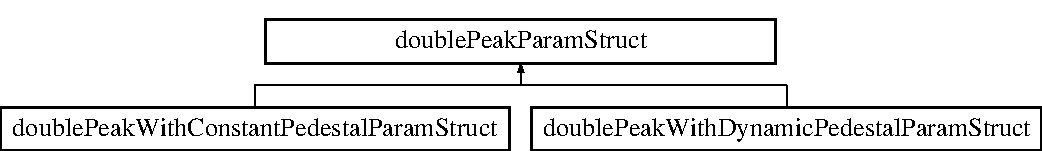
\includegraphics[height=2.000000cm]{structdouble_peak_param_struct}
\end{center}
\end{figure}
\subsection*{Public Member Functions}
\begin{DoxyCompactItemize}
\item 
\hypertarget{structdouble_peak_param_struct_aeb34f180e50540e55ee7e5a3ff27634d}{}{\bfseries double\+Peak\+Param\+Struct} (Double\+\_\+t shifted\+Time\+First\+Peak, Double\+\_\+t scaling\+Factor\+First\+Peak, Double\+\_\+t shifted\+Time\+Second\+Peak, Double\+\_\+t scaling\+Factor\+Second\+Peak)\label{structdouble_peak_param_struct_aeb34f180e50540e55ee7e5a3ff27634d}

\end{DoxyCompactItemize}
\subsection*{Public Attributes}
\begin{DoxyCompactItemize}
\item 
\hypertarget{structdouble_peak_param_struct_a9dd38f714912463e1dfc64b95db3988b}{}Double\+\_\+t {\bfseries \+\_\+shifted\+Time\+First\+Peak}\label{structdouble_peak_param_struct_a9dd38f714912463e1dfc64b95db3988b}

\item 
\hypertarget{structdouble_peak_param_struct_abc363790ee7e6eccac70d92306cb7d19}{}Double\+\_\+t {\bfseries \+\_\+scaling\+Factor\+First\+Peak}\label{structdouble_peak_param_struct_abc363790ee7e6eccac70d92306cb7d19}

\item 
\hypertarget{structdouble_peak_param_struct_a3cc0e97fd5dd9edc2a5b0caeb1ebcf97}{}Double\+\_\+t {\bfseries \+\_\+shifted\+Time\+Second\+Peak}\label{structdouble_peak_param_struct_a3cc0e97fd5dd9edc2a5b0caeb1ebcf97}

\item 
\hypertarget{structdouble_peak_param_struct_a3213e45bb4aa8f588fb605d70155e85c}{}Double\+\_\+t {\bfseries \+\_\+scaling\+Factor\+Second\+Peak}\label{structdouble_peak_param_struct_a3213e45bb4aa8f588fb605d70155e85c}

\end{DoxyCompactItemize}


The documentation for this struct was generated from the following file\+:\begin{DoxyCompactItemize}
\item 
Param\+Structs.\+hh\end{DoxyCompactItemize}

\hypertarget{structdouble_peak_with_constant_pedestal_param_struct}{}\section{double\+Peak\+With\+Constant\+Pedestal\+Param\+Struct Struct Reference}
\label{structdouble_peak_with_constant_pedestal_param_struct}\index{double\+Peak\+With\+Constant\+Pedestal\+Param\+Struct@{double\+Peak\+With\+Constant\+Pedestal\+Param\+Struct}}
Inheritance diagram for double\+Peak\+With\+Constant\+Pedestal\+Param\+Struct\+:\begin{figure}[H]
\begin{center}
\leavevmode
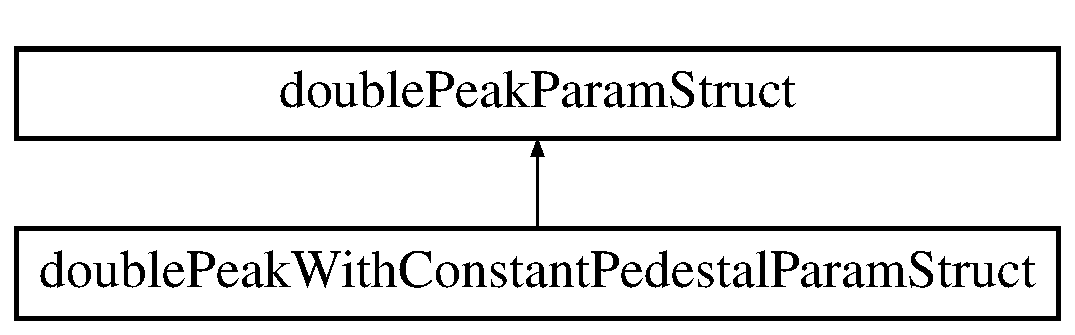
\includegraphics[height=2.000000cm]{structdouble_peak_with_constant_pedestal_param_struct}
\end{center}
\end{figure}
\subsection*{Public Member Functions}
\begin{DoxyCompactItemize}
\item 
\hypertarget{structdouble_peak_with_constant_pedestal_param_struct_ab7a85f3cee2363af395a7c295ecd648c}{}{\bfseries double\+Peak\+With\+Constant\+Pedestal\+Param\+Struct} (Double\+\_\+t shifted\+Time\+First\+Peak, Double\+\_\+t scaling\+Factor\+First\+Peak, Double\+\_\+t vertical\+Shift, Double\+\_\+t shifted\+Time\+Second\+Peak, Double\+\_\+t scaling\+Factor\+Second\+Peak)\label{structdouble_peak_with_constant_pedestal_param_struct_ab7a85f3cee2363af395a7c295ecd648c}

\end{DoxyCompactItemize}
\subsection*{Public Attributes}
\begin{DoxyCompactItemize}
\item 
\hypertarget{structdouble_peak_with_constant_pedestal_param_struct_a8d42a7e7318a458ec1639988051153b3}{}Double\+\_\+t {\bfseries \+\_\+vertical\+Shift}\label{structdouble_peak_with_constant_pedestal_param_struct_a8d42a7e7318a458ec1639988051153b3}

\end{DoxyCompactItemize}


The documentation for this struct was generated from the following file\+:\begin{DoxyCompactItemize}
\item 
Param\+Structs.\+hh\end{DoxyCompactItemize}

\hypertarget{structdouble_peak_with_dynamic_pedestal_param_struct}{}\section{double\+Peak\+With\+Dynamic\+Pedestal\+Param\+Struct Struct Reference}
\label{structdouble_peak_with_dynamic_pedestal_param_struct}\index{double\+Peak\+With\+Dynamic\+Pedestal\+Param\+Struct@{double\+Peak\+With\+Dynamic\+Pedestal\+Param\+Struct}}
Inheritance diagram for double\+Peak\+With\+Dynamic\+Pedestal\+Param\+Struct\+:\begin{figure}[H]
\begin{center}
\leavevmode
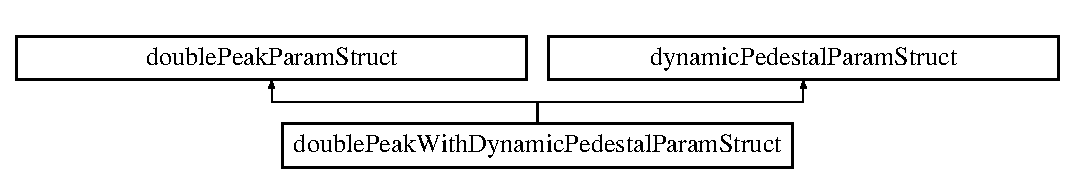
\includegraphics[height=2.000000cm]{structdouble_peak_with_dynamic_pedestal_param_struct}
\end{center}
\end{figure}
\subsection*{Public Member Functions}
\begin{DoxyCompactItemize}
\item 
\hypertarget{structdouble_peak_with_dynamic_pedestal_param_struct_abb78e48a8a4e432b051e411c058e6e36}{}{\bfseries double\+Peak\+With\+Dynamic\+Pedestal\+Param\+Struct} (Double\+\_\+t shifted\+Time\+First\+Peak, Double\+\_\+t scaling\+Factor\+First\+Peak, Double\+\_\+t Q, Double\+\_\+t shifted\+Time\+Second\+Peak, Double\+\_\+t scaling\+Factor\+Second\+Peak)\label{structdouble_peak_with_dynamic_pedestal_param_struct_abb78e48a8a4e432b051e411c058e6e36}

\end{DoxyCompactItemize}
\subsection*{Additional Inherited Members}


The documentation for this struct was generated from the following file\+:\begin{DoxyCompactItemize}
\item 
Param\+Structs.\+hh\end{DoxyCompactItemize}

\hypertarget{structdynamic_pedestal_param_struct}{}\section{dynamic\+Pedestal\+Param\+Struct Struct Reference}
\label{structdynamic_pedestal_param_struct}\index{dynamic\+Pedestal\+Param\+Struct@{dynamic\+Pedestal\+Param\+Struct}}
Inheritance diagram for dynamic\+Pedestal\+Param\+Struct\+:\begin{figure}[H]
\begin{center}
\leavevmode
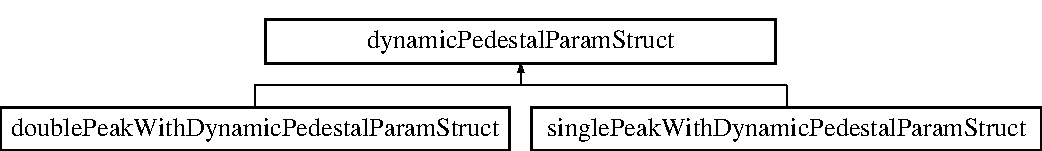
\includegraphics[height=2.000000cm]{structdynamic_pedestal_param_struct}
\end{center}
\end{figure}
\subsection*{Public Member Functions}
\begin{DoxyCompactItemize}
\item 
\hypertarget{structdynamic_pedestal_param_struct_a7ffeca608a7b6c23b4d8fbf890b7083a}{}{\bfseries dynamic\+Pedestal\+Param\+Struct} (Double\+\_\+t Q)\label{structdynamic_pedestal_param_struct_a7ffeca608a7b6c23b4d8fbf890b7083a}

\end{DoxyCompactItemize}
\subsection*{Public Attributes}
\begin{DoxyCompactItemize}
\item 
\hypertarget{structdynamic_pedestal_param_struct_a50bb36d950b91597e5a159ceaaa9e7c0}{}Double\+\_\+t {\bfseries \+\_\+\+Q}\label{structdynamic_pedestal_param_struct_a50bb36d950b91597e5a159ceaaa9e7c0}

\end{DoxyCompactItemize}


The documentation for this struct was generated from the following file\+:\begin{DoxyCompactItemize}
\item 
Param\+Structs.\+hh\end{DoxyCompactItemize}

\hypertarget{class_find_double_peak}{}\section{Find\+Double\+Peak Class Reference}
\label{class_find_double_peak}\index{Find\+Double\+Peak@{Find\+Double\+Peak}}
Inheritance diagram for Find\+Double\+Peak\+:\begin{figure}[H]
\begin{center}
\leavevmode
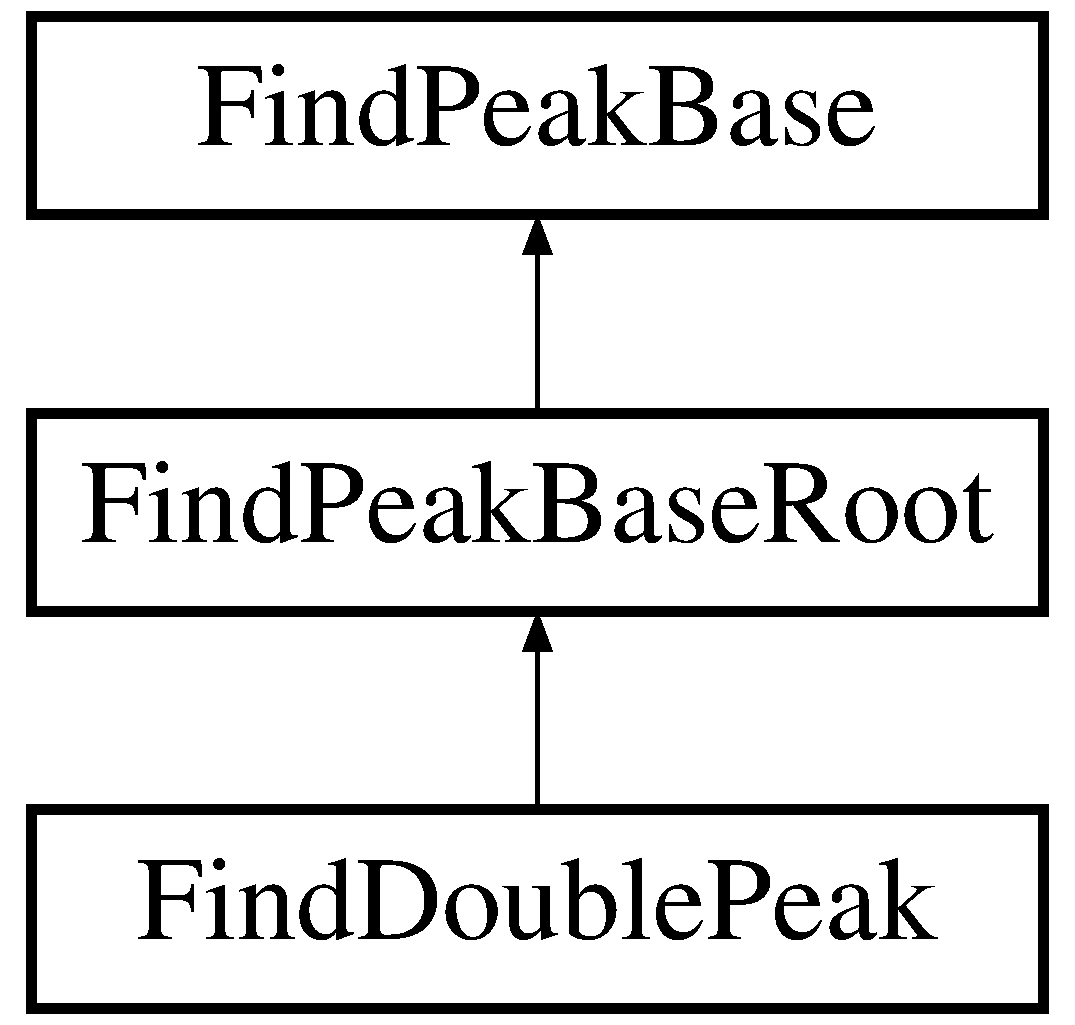
\includegraphics[height=3.000000cm]{class_find_double_peak}
\end{center}
\end{figure}
\subsection*{Public Member Functions}
\begin{DoxyCompactItemize}
\item 
\hypertarget{class_find_double_peak_a3e553252c23fe24121eb352db128ea2b}{}{\bfseries Find\+Double\+Peak} (const \hyperlink{structconfig_struct}{config\+Struct} \&init\+Params)\label{class_find_double_peak_a3e553252c23fe24121eb352db128ea2b}

\item 
\hypertarget{class_find_double_peak_a4ab15919d094e8aff35ffbda61d8d145}{}virtual void {\bfseries process} (const adc\+Waveform adc\+Data, resultant\+Hit\+Data \&result)\label{class_find_double_peak_a4ab15919d094e8aff35ffbda61d8d145}

\end{DoxyCompactItemize}
\subsection*{Protected Member Functions}
\begin{DoxyCompactItemize}
\item 
\hypertarget{class_find_double_peak_ab477eb13e047e74d8a491670da899122}{}void {\bfseries fit\+Params2\+Resultant\+Data} (const Double\+\_\+t $\ast$fit\+Parameters, resultant\+Hit\+Data \&result)\label{class_find_double_peak_ab477eb13e047e74d8a491670da899122}

\end{DoxyCompactItemize}
\subsection*{Additional Inherited Members}


The documentation for this class was generated from the following files\+:\begin{DoxyCompactItemize}
\item 
Find\+Multiple\+Peak.\+hh\item 
Find\+Multiple\+Peak.\+cc\end{DoxyCompactItemize}

\hypertarget{class_find_double_peak_with_dynamic_pedestal}{}\section{Find\+Double\+Peak\+With\+Dynamic\+Pedestal Class Reference}
\label{class_find_double_peak_with_dynamic_pedestal}\index{Find\+Double\+Peak\+With\+Dynamic\+Pedestal@{Find\+Double\+Peak\+With\+Dynamic\+Pedestal}}
Inheritance diagram for Find\+Double\+Peak\+With\+Dynamic\+Pedestal\+:\begin{figure}[H]
\begin{center}
\leavevmode
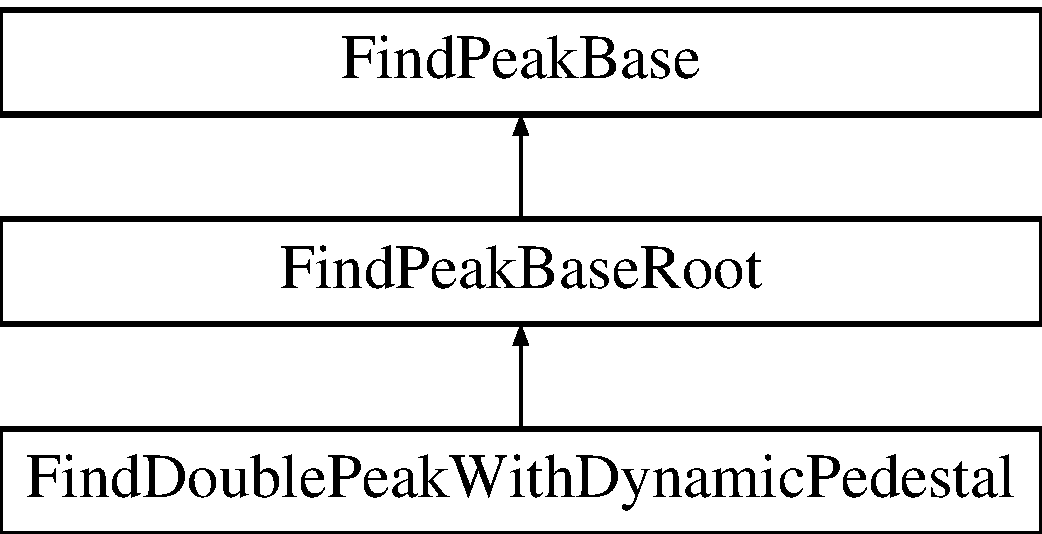
\includegraphics[height=3.000000cm]{class_find_double_peak_with_dynamic_pedestal}
\end{center}
\end{figure}
\subsection*{Public Member Functions}
\begin{DoxyCompactItemize}
\item 
\hypertarget{class_find_double_peak_with_dynamic_pedestal_a3e911ccbe5da00980b273e7e063b06e9}{}{\bfseries Find\+Double\+Peak\+With\+Dynamic\+Pedestal} (const \hyperlink{structconfig_struct}{config\+Struct} \&init\+Params)\label{class_find_double_peak_with_dynamic_pedestal_a3e911ccbe5da00980b273e7e063b06e9}

\item 
\hypertarget{class_find_double_peak_with_dynamic_pedestal_a36ebd5c56d243eaf14b65775059306c0}{}virtual void {\bfseries process} (const adc\+Waveform adc\+Data, resultant\+Hit\+Data \&result)\label{class_find_double_peak_with_dynamic_pedestal_a36ebd5c56d243eaf14b65775059306c0}

\end{DoxyCompactItemize}
\subsection*{Additional Inherited Members}


The documentation for this class was generated from the following files\+:\begin{DoxyCompactItemize}
\item 
Find\+Multiple\+Peak.\+hh\item 
Find\+Multiple\+Peak.\+cc\end{DoxyCompactItemize}

\hypertarget{class_find_multiple_peaks}{}\section{Find\+Multiple\+Peaks Class Reference}
\label{class_find_multiple_peaks}\index{Find\+Multiple\+Peaks@{Find\+Multiple\+Peaks}}
Inheritance diagram for Find\+Multiple\+Peaks\+:\begin{figure}[H]
\begin{center}
\leavevmode
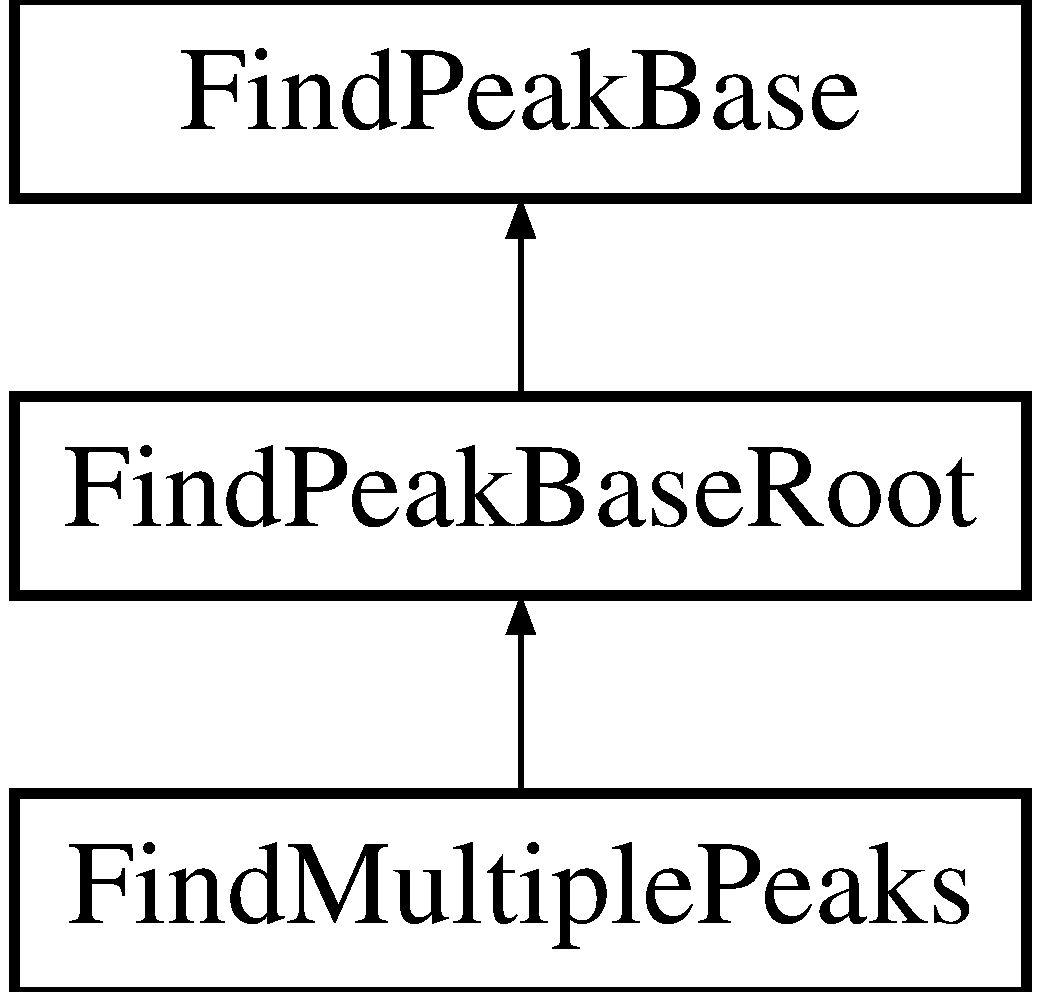
\includegraphics[height=3.000000cm]{class_find_multiple_peaks}
\end{center}
\end{figure}
\subsection*{Public Member Functions}
\begin{DoxyCompactItemize}
\item 
\hypertarget{class_find_multiple_peaks_ae0fd95088520b85c5c02ae182241c2da}{}{\bfseries Find\+Multiple\+Peaks} (const \hyperlink{structconfig_struct}{config\+Struct} \&init\+Params)\label{class_find_multiple_peaks_ae0fd95088520b85c5c02ae182241c2da}

\item 
\hypertarget{class_find_multiple_peaks_a26011d385dff3edd1dd818862bcf6c5d}{}virtual void {\bfseries process} (const adc\+Waveform adc\+Data, resultant\+Hit\+Data \&result)\label{class_find_multiple_peaks_a26011d385dff3edd1dd818862bcf6c5d}

\end{DoxyCompactItemize}
\subsection*{Additional Inherited Members}


The documentation for this class was generated from the following files\+:\begin{DoxyCompactItemize}
\item 
Find\+Multiple\+Peak.\+hh\item 
Find\+Multiple\+Peak.\+cc\end{DoxyCompactItemize}

\hypertarget{class_find_peak_base}{}\section{Find\+Peak\+Base Class Reference}
\label{class_find_peak_base}\index{Find\+Peak\+Base@{Find\+Peak\+Base}}


{\ttfamily \#include $<$Find\+Peak\+Base.\+hh$>$}

Inheritance diagram for Find\+Peak\+Base\+:\begin{figure}[H]
\begin{center}
\leavevmode
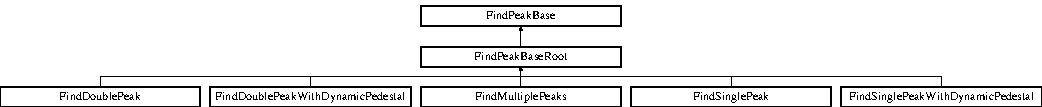
\includegraphics[height=1.435897cm]{class_find_peak_base}
\end{center}
\end{figure}
\subsection*{Public Member Functions}
\begin{DoxyCompactItemize}
\item 
\hypertarget{class_find_peak_base_a59ec4911e522e1814a052ffa7d8f46f8}{}virtual void {\bfseries process} (const adc\+Waveform adc\+Data, resultant\+Hit\+Data \&result)=0\label{class_find_peak_base_a59ec4911e522e1814a052ffa7d8f46f8}

\item 
\hypertarget{class_find_peak_base_a8d291602ae052dcf9f9c15c818400c43}{}{\bfseries Find\+Peak\+Base} (const \hyperlink{structconfig_struct}{config\+Struct} \&init\+Params)\label{class_find_peak_base_a8d291602ae052dcf9f9c15c818400c43}

\end{DoxyCompactItemize}
\subsection*{Protected Attributes}
\begin{DoxyCompactItemize}
\item 
\hypertarget{class_find_peak_base_af020ca3bc5ab34bde76382150e06c558}{}\hyperlink{structconfig_struct}{config\+Struct} {\bfseries \+\_\+init\+Params}\label{class_find_peak_base_af020ca3bc5ab34bde76382150e06c558}

\item 
\hypertarget{class_find_peak_base_a1dd81b2aed6ceff885cd371dbe23b9cb}{}const Double\+\_\+t {\bfseries \+\_\+bits2scaling\+Factor}\label{class_find_peak_base_a1dd81b2aed6ceff885cd371dbe23b9cb}

\item 
\hypertarget{class_find_peak_base_aeacee514c100fe4def492565ab20ef5d}{}const Double\+\_\+t {\bfseries \+\_\+scaling\+Factor2bits}\label{class_find_peak_base_aeacee514c100fe4def492565ab20ef5d}

\item 
\hypertarget{class_find_peak_base_a23da473fdf06ed61af98530dd6a9e231}{}const Double\+\_\+t {\bfseries \+\_\+hit\+Period}\label{class_find_peak_base_a23da473fdf06ed61af98530dd6a9e231}

\end{DoxyCompactItemize}


\subsection{Detailed Description}
Virtual class providing structure for \hyperlink{class_find_single_peak}{Find\+Single\+Peak}, \hyperlink{class_find_double_peak}{Find\+Double\+Peak}, Find\+Mutiple\+Peaks, etc. 

The documentation for this class was generated from the following file\+:\begin{DoxyCompactItemize}
\item 
Find\+Peak\+Base.\+hh\end{DoxyCompactItemize}

\hypertarget{class_find_peak_base_root}{}\section{Find\+Peak\+Base\+Root Class Reference}
\label{class_find_peak_base_root}\index{Find\+Peak\+Base\+Root@{Find\+Peak\+Base\+Root}}
Inheritance diagram for Find\+Peak\+Base\+Root\+:\begin{figure}[H]
\begin{center}
\leavevmode
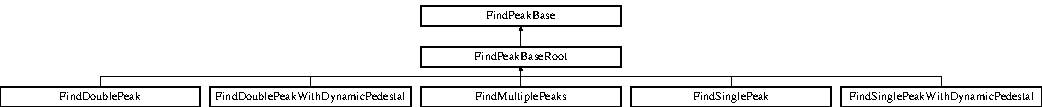
\includegraphics[height=1.435897cm]{class_find_peak_base_root}
\end{center}
\end{figure}
\subsection*{Public Member Functions}
\begin{DoxyCompactItemize}
\item 
\hypertarget{class_find_peak_base_root_a1fbcb56012580740749309aa8d51d6ae}{}virtual void {\bfseries process} (const adc\+Waveform adc\+Data, resultant\+Hit\+Data \&result)=0\label{class_find_peak_base_root_a1fbcb56012580740749309aa8d51d6ae}

\item 
\hypertarget{class_find_peak_base_root_a10c62343b210464b163cc54fc1ef4a6b}{}{\bfseries Find\+Peak\+Base\+Root} (const \hyperlink{structconfig_struct}{config\+Struct} \&init\+Params)\label{class_find_peak_base_root_a10c62343b210464b163cc54fc1ef4a6b}

\end{DoxyCompactItemize}
\subsection*{Protected Member Functions}
\begin{DoxyCompactItemize}
\item 
\hypertarget{class_find_peak_base_root_aabc241ad84eb6945c86a47aad9f19e99}{}void {\bfseries fit\+Model2\+Normalized\+Waveform} (T\+F1 \&fit\+Model, T\+Graph\+Errors \&fit\+Data, const Double\+\_\+t $\ast$initial\+Parameters, Double\+\_\+t $\ast$fit\+Parameters)\label{class_find_peak_base_root_aabc241ad84eb6945c86a47aad9f19e99}

\item 
\hypertarget{class_find_peak_base_root_aaa4f0593f5a30f1f4c91b9325f3a24ac}{}void {\bfseries adc\+Waveform2\+T\+Graph\+Errors} (adc\+Waveform adc\+Data, T\+Graph\+Errors \&fit\+Data)\label{class_find_peak_base_root_aaa4f0593f5a30f1f4c91b9325f3a24ac}

\end{DoxyCompactItemize}
\subsection*{Additional Inherited Members}


The documentation for this class was generated from the following files\+:\begin{DoxyCompactItemize}
\item 
Find\+Peak\+Base\+Root.\+hh\item 
Find\+Peak\+Base\+Root.\+cc\end{DoxyCompactItemize}

\hypertarget{class_find_single_peak}{}\section{Find\+Single\+Peak Class Reference}
\label{class_find_single_peak}\index{Find\+Single\+Peak@{Find\+Single\+Peak}}
Inheritance diagram for Find\+Single\+Peak\+:\begin{figure}[H]
\begin{center}
\leavevmode
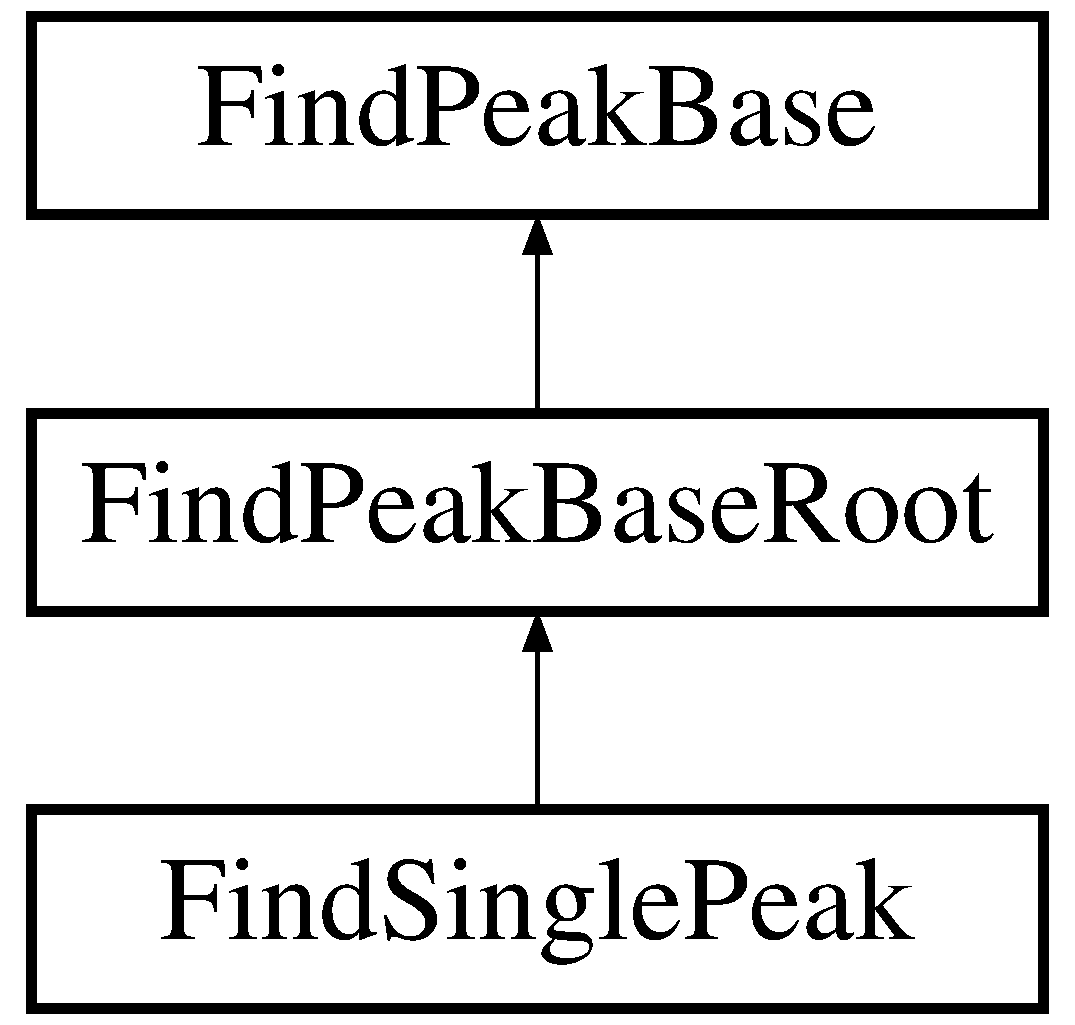
\includegraphics[height=3.000000cm]{class_find_single_peak}
\end{center}
\end{figure}
\subsection*{Public Member Functions}
\begin{DoxyCompactItemize}
\item 
\hypertarget{class_find_single_peak_a5453373fe5dcd2b562a6196c1f672962}{}{\bfseries Find\+Single\+Peak} (const \hyperlink{structconfig_struct}{config\+Struct} \&init\+Params)\label{class_find_single_peak_a5453373fe5dcd2b562a6196c1f672962}

\item 
\hypertarget{class_find_single_peak_a1c51746e44a2c72981b45891128c3847}{}virtual void {\bfseries process} (const adc\+Waveform adc\+Data, resultant\+Hit\+Data \&result)\label{class_find_single_peak_a1c51746e44a2c72981b45891128c3847}

\end{DoxyCompactItemize}
\subsection*{Additional Inherited Members}


The documentation for this class was generated from the following files\+:\begin{DoxyCompactItemize}
\item 
Find\+Multiple\+Peak.\+hh\item 
Find\+Multiple\+Peak.\+cc\end{DoxyCompactItemize}

\hypertarget{class_find_single_peak_with_dynamic_pedestal}{}\section{Find\+Single\+Peak\+With\+Dynamic\+Pedestal Class Reference}
\label{class_find_single_peak_with_dynamic_pedestal}\index{Find\+Single\+Peak\+With\+Dynamic\+Pedestal@{Find\+Single\+Peak\+With\+Dynamic\+Pedestal}}
Inheritance diagram for Find\+Single\+Peak\+With\+Dynamic\+Pedestal\+:\begin{figure}[H]
\begin{center}
\leavevmode
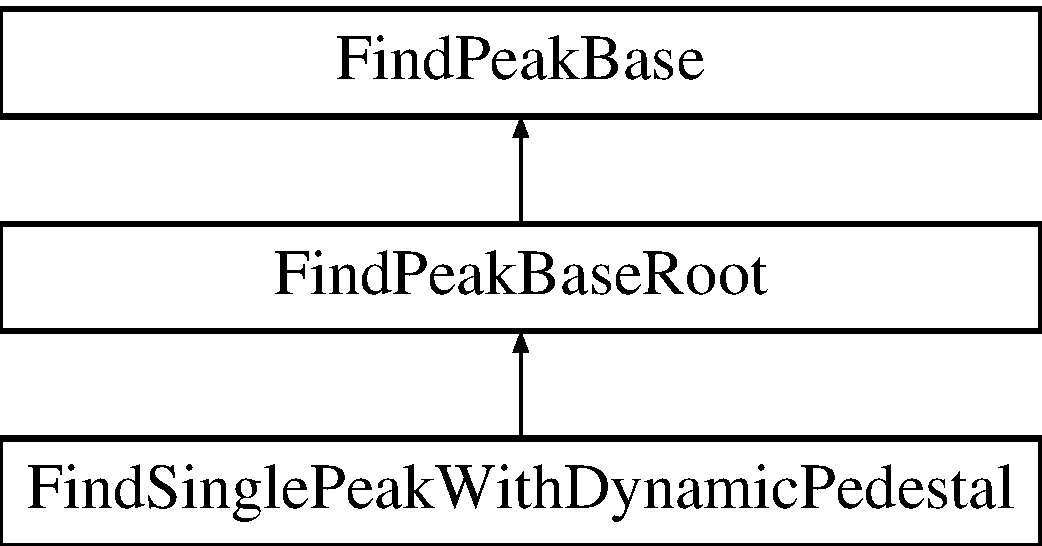
\includegraphics[height=3.000000cm]{class_find_single_peak_with_dynamic_pedestal}
\end{center}
\end{figure}
\subsection*{Public Member Functions}
\begin{DoxyCompactItemize}
\item 
\hypertarget{class_find_single_peak_with_dynamic_pedestal_a620e1d3264f0f939e47130bf239cc04f}{}{\bfseries Find\+Single\+Peak\+With\+Dynamic\+Pedestal} (const \hyperlink{structconfig_struct}{config\+Struct} \&init\+Params)\label{class_find_single_peak_with_dynamic_pedestal_a620e1d3264f0f939e47130bf239cc04f}

\item 
\hypertarget{class_find_single_peak_with_dynamic_pedestal_a4dc2eb2fbdb3463046c26baa90f35833}{}virtual void {\bfseries process} (const adc\+Waveform adc\+Data, resultant\+Hit\+Data \&result)\label{class_find_single_peak_with_dynamic_pedestal_a4dc2eb2fbdb3463046c26baa90f35833}

\end{DoxyCompactItemize}
\subsection*{Additional Inherited Members}


The documentation for this class was generated from the following files\+:\begin{DoxyCompactItemize}
\item 
Find\+Multiple\+Peak.\+hh\item 
Find\+Multiple\+Peak.\+cc\end{DoxyCompactItemize}

\hypertarget{structresultant_peak_data}{}\section{resultant\+Peak\+Data Struct Reference}
\label{structresultant_peak_data}\index{resultant\+Peak\+Data@{resultant\+Peak\+Data}}
\subsection*{Public Member Functions}
\begin{DoxyCompactItemize}
\item 
\hypertarget{structresultant_peak_data_a33b55c24f503ffd5e341b52105bd9e4b}{}{\bfseries resultant\+Peak\+Data} (Float\+\_\+t peak\+Time, Float\+\_\+t peak\+Height)\label{structresultant_peak_data_a33b55c24f503ffd5e341b52105bd9e4b}

\end{DoxyCompactItemize}
\subsection*{Public Attributes}
\begin{DoxyCompactItemize}
\item 
\hypertarget{structresultant_peak_data_abc8f4ed26aa12bd0a9b49527f7599c3b}{}Float\+\_\+t {\bfseries \+\_\+peak\+Height}\label{structresultant_peak_data_abc8f4ed26aa12bd0a9b49527f7599c3b}

\item 
\hypertarget{structresultant_peak_data_aac009547ef6ed9044d06d95a9dae9ce5}{}Float\+\_\+t {\bfseries \+\_\+peak\+Time}\label{structresultant_peak_data_aac009547ef6ed9044d06d95a9dae9ce5}

\end{DoxyCompactItemize}


The documentation for this struct was generated from the following file\+:\begin{DoxyCompactItemize}
\item 
Find\+Peak\+Base.\+hh\end{DoxyCompactItemize}

\hypertarget{structsingle_peak_param_struct}{}\section{single\+Peak\+Param\+Struct Struct Reference}
\label{structsingle_peak_param_struct}\index{single\+Peak\+Param\+Struct@{single\+Peak\+Param\+Struct}}
Inheritance diagram for single\+Peak\+Param\+Struct\+:\begin{figure}[H]
\begin{center}
\leavevmode
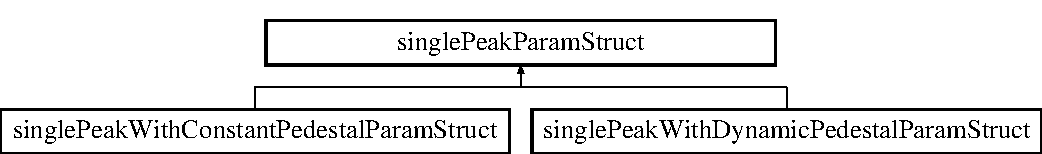
\includegraphics[height=2.000000cm]{structsingle_peak_param_struct}
\end{center}
\end{figure}
\subsection*{Public Member Functions}
\begin{DoxyCompactItemize}
\item 
\hypertarget{structsingle_peak_param_struct_acdd82f9fe9a24d725c672509f7cff025}{}{\bfseries single\+Peak\+Param\+Struct} (Double\+\_\+t shifted\+Time, Double\+\_\+t scaling\+Factor, Double\+\_\+t sigma=0.\+0)\label{structsingle_peak_param_struct_acdd82f9fe9a24d725c672509f7cff025}

\end{DoxyCompactItemize}
\subsection*{Public Attributes}
\begin{DoxyCompactItemize}
\item 
\hypertarget{structsingle_peak_param_struct_aae2389f2da24586e2fd21ce38b33edd1}{}Double\+\_\+t {\bfseries \+\_\+shifted\+Time}\label{structsingle_peak_param_struct_aae2389f2da24586e2fd21ce38b33edd1}

\item 
\hypertarget{structsingle_peak_param_struct_a72d0a676851e57dd6c336df4ae4cf61d}{}Double\+\_\+t {\bfseries \+\_\+scaling\+Factor}\label{structsingle_peak_param_struct_a72d0a676851e57dd6c336df4ae4cf61d}

\item 
\hypertarget{structsingle_peak_param_struct_a323e63c0fe70f09f342080c7a6736ad8}{}Double\+\_\+t {\bfseries \+\_\+sigma}\label{structsingle_peak_param_struct_a323e63c0fe70f09f342080c7a6736ad8}

\end{DoxyCompactItemize}


The documentation for this struct was generated from the following file\+:\begin{DoxyCompactItemize}
\item 
Param\+Structs.\+hh\end{DoxyCompactItemize}

\hypertarget{structsingle_peak_with_constant_pedestal_param_struct}{}\section{single\+Peak\+With\+Constant\+Pedestal\+Param\+Struct Struct Reference}
\label{structsingle_peak_with_constant_pedestal_param_struct}\index{single\+Peak\+With\+Constant\+Pedestal\+Param\+Struct@{single\+Peak\+With\+Constant\+Pedestal\+Param\+Struct}}
Inheritance diagram for single\+Peak\+With\+Constant\+Pedestal\+Param\+Struct\+:\begin{figure}[H]
\begin{center}
\leavevmode
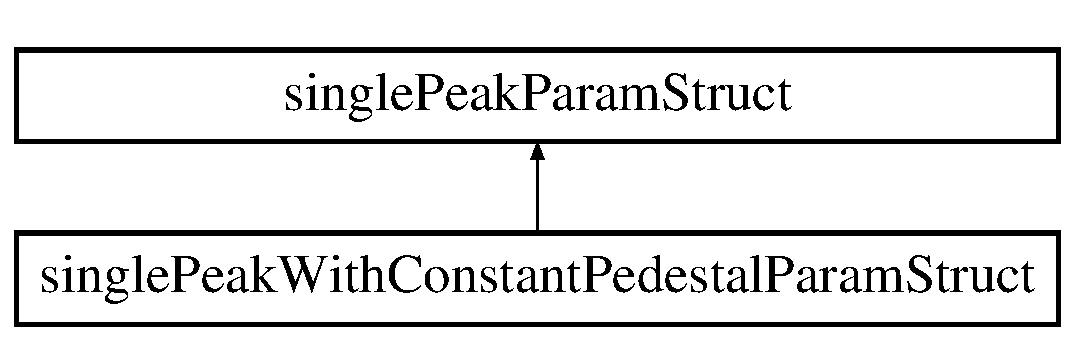
\includegraphics[height=2.000000cm]{structsingle_peak_with_constant_pedestal_param_struct}
\end{center}
\end{figure}
\subsection*{Public Member Functions}
\begin{DoxyCompactItemize}
\item 
\hypertarget{structsingle_peak_with_constant_pedestal_param_struct_a7c214c75ae764ac1f82dd0d384ba8e41}{}{\bfseries single\+Peak\+With\+Constant\+Pedestal\+Param\+Struct} (Double\+\_\+t shifted\+Time, Double\+\_\+t scaling\+Factor, Double\+\_\+t vertical\+Shift, Double\+\_\+t sigma)\label{structsingle_peak_with_constant_pedestal_param_struct_a7c214c75ae764ac1f82dd0d384ba8e41}

\end{DoxyCompactItemize}
\subsection*{Public Attributes}
\begin{DoxyCompactItemize}
\item 
\hypertarget{structsingle_peak_with_constant_pedestal_param_struct_ad062c199965b3e1e920075deba7d150a}{}Double\+\_\+t {\bfseries \+\_\+vertical\+Shift}\label{structsingle_peak_with_constant_pedestal_param_struct_ad062c199965b3e1e920075deba7d150a}

\end{DoxyCompactItemize}


The documentation for this struct was generated from the following file\+:\begin{DoxyCompactItemize}
\item 
Param\+Structs.\+hh\end{DoxyCompactItemize}

\hypertarget{structsingle_peak_with_dynamic_pedestal_param_struct}{}\section{single\+Peak\+With\+Dynamic\+Pedestal\+Param\+Struct Struct Reference}
\label{structsingle_peak_with_dynamic_pedestal_param_struct}\index{single\+Peak\+With\+Dynamic\+Pedestal\+Param\+Struct@{single\+Peak\+With\+Dynamic\+Pedestal\+Param\+Struct}}
Inheritance diagram for single\+Peak\+With\+Dynamic\+Pedestal\+Param\+Struct\+:\begin{figure}[H]
\begin{center}
\leavevmode
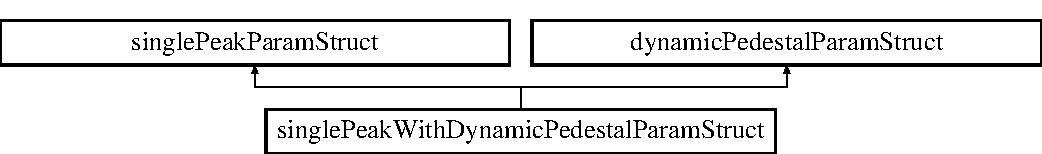
\includegraphics[height=2.000000cm]{structsingle_peak_with_dynamic_pedestal_param_struct}
\end{center}
\end{figure}
\subsection*{Public Member Functions}
\begin{DoxyCompactItemize}
\item 
\hypertarget{structsingle_peak_with_dynamic_pedestal_param_struct_a8626ce58ea8b85e97cfc8d6a94ec4b92}{}{\bfseries single\+Peak\+With\+Dynamic\+Pedestal\+Param\+Struct} (Double\+\_\+t shifted\+Time, Double\+\_\+t scaling\+Factor, Double\+\_\+t Q, Double\+\_\+t sigma)\label{structsingle_peak_with_dynamic_pedestal_param_struct_a8626ce58ea8b85e97cfc8d6a94ec4b92}

\end{DoxyCompactItemize}
\subsection*{Additional Inherited Members}


The documentation for this struct was generated from the following file\+:\begin{DoxyCompactItemize}
\item 
Param\+Structs.\+hh\end{DoxyCompactItemize}

%--- End generated contents ---

% Index
\backmatter
\newpage
\phantomsection
\clearemptydoublepage
\addcontentsline{toc}{chapter}{Index}
\printindex

\end{document}
